\documentclass{beamer}

\usetheme{Madrid}
\usecolortheme{spruce}

\usepackage{graphicx}
\graphicspath{{./img/}}

\title{Management Application of an Agent-Based Model: Control of Cowbirds at
the Landscape Level}
\subtitle{Harper, Westervelt, and Shapiro (2002)}
\author{Tom Wallace}
\institute{George Mason University}
\date{Spring 2018}

\begin{document}

\frame{\titlepage}

\begin{frame}
	\frametitle{The greatest threats to the United States?}
	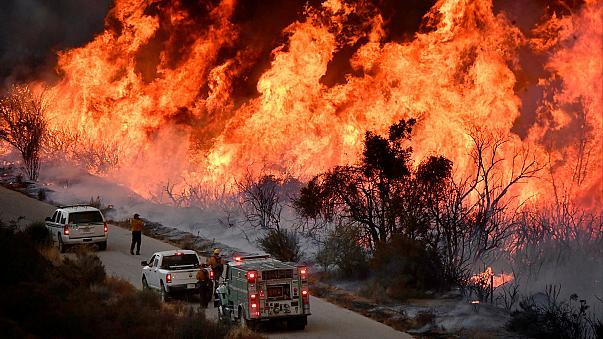
\includegraphics[height=1.5in, keepaspectratio]{fire.jpg}
	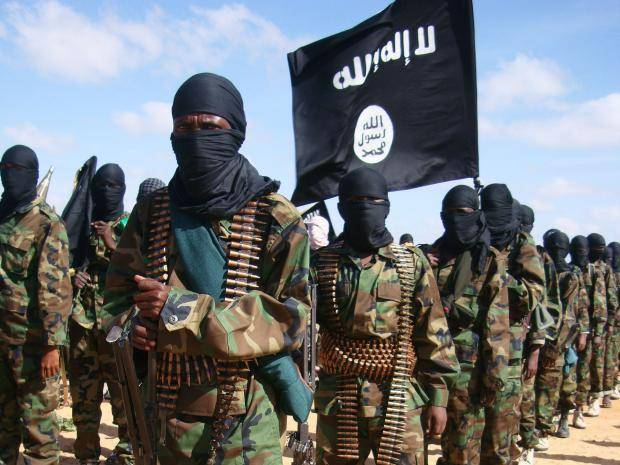
\includegraphics[height=1.5in, keepaspectratio]{terrorists.jpg}
	
\includegraphics[height=1.5in, keepaspectratio]{collapse.jpeg}
\end{frame}

\begin{frame}
	\frametitle{The hidden menace}
	\begin{center}
		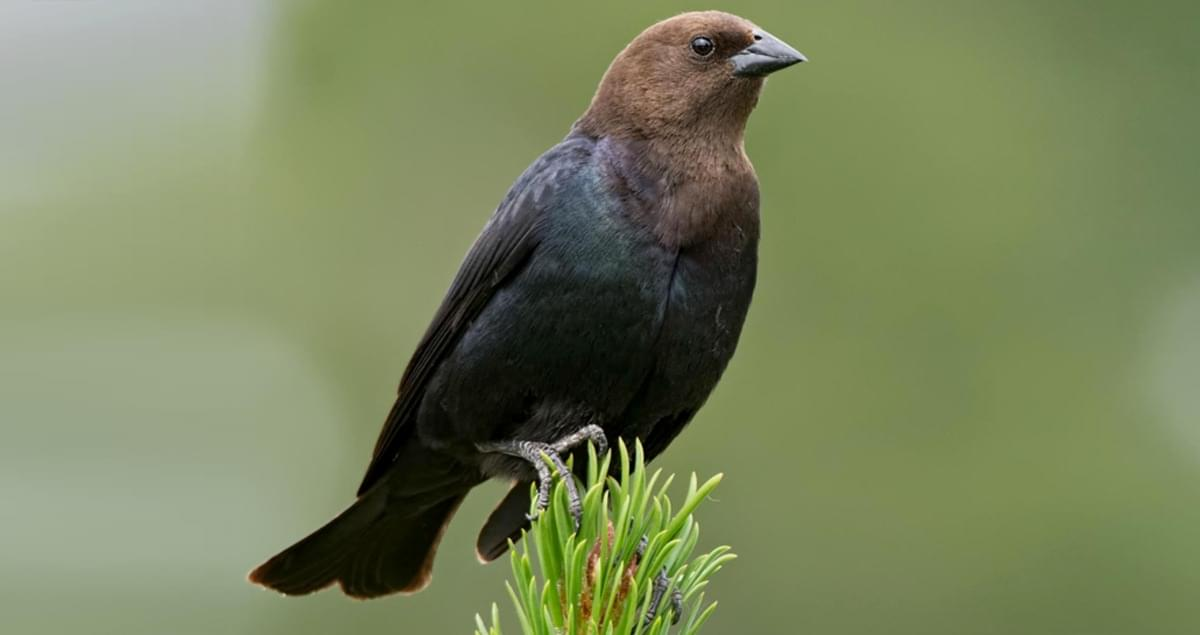
\includegraphics[height=2.5in, keepaspectratio]{bird.jpg}
	\end{center}
\end{frame}

\begin{frame}
	\frametitle{A bloody campaign of deception and sabotage}
	\begin{center}
		\includegraphics[height=1.5in, keepaspectratio]{nest.jpg}
		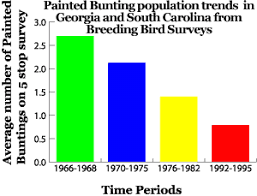
\includegraphics[height=1.5in, keepaspectratio]{trend.png}
	\end{center}
\end{frame}

\begin{frame}
	\frametitle{Taking aim at the heart of American military power}
	\begin{center}
		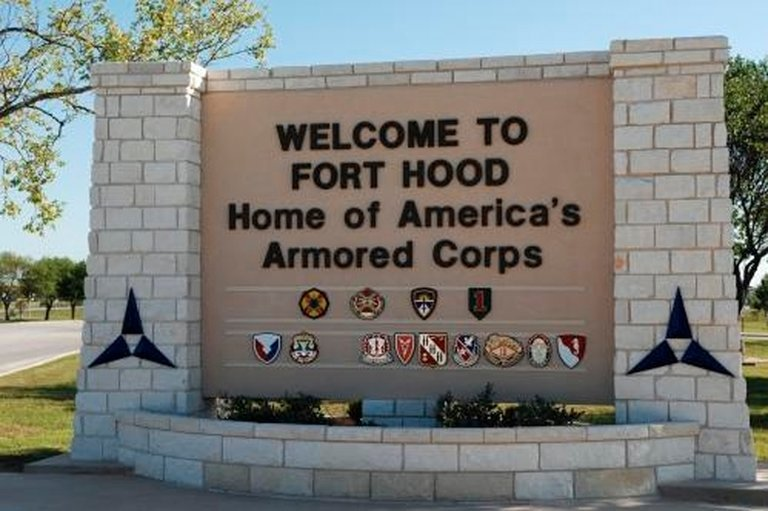
\includegraphics[height=1.5in, keepaspectratio]{fort.jpg}
		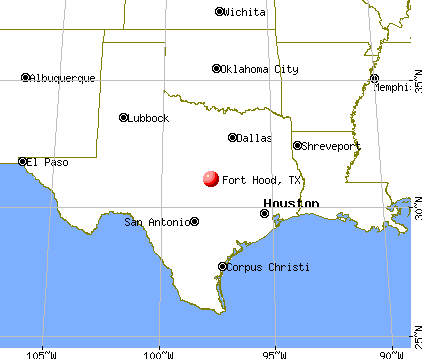
\includegraphics[height=1.5in, keepaspectratio]{map.png}
	\end{center}
\end{frame}

\begin{frame}
	\frametitle{Only the A(BM)-Team can stop this reign of terror}
		Authors
			\begin{itemize}
				\item \small Steven Harper, University of Georgia
				\item \small James Westervelt, U.S. Army Corps of Engineers
				\item \small Ann-Marie Shapiro, University of Illinois
					\\~\\
			\end{itemize}
		Other research
			\begin{itemize}
				\item \small Desert tortoises at Fort Irwin
				\item \small Endangered birds at Fort Hood \\~\\
			\end{itemize}

		Goals
			\begin{itemize}
				\item \small Build model to predict feeding locations of cowbirds
				\item \small Extend model to simulate trapping of cowbirds
				\item \small Use this capability to develop optimal trapping strategy
				\item \small Terminate with extreme prejudice
			\end{itemize}
\end{frame}

\begin{frame}
	\frametitle{Overview}
	GIS (GRASS) and ABM (SWARM) \\~\\

	58 km x 58 km (335,000 ha) area \\~\\

	1 day time step, 100 steps \\~\\

	Three agent types
	\begin{itemize}
		\item \small Feeding area (fixed)
		\item \small Cattle herd (mobile)
		\item \small Cowbird (mobile) \\~\\
	\end{itemize}

	Feeding area $\to$ cattle movement $\to$ bird movement $\to$ trap placement

\end{frame}

\begin{frame}
	\frametitle{Feeding areas}
	56 ha square \\~\\

	Main attribute of interest: \textbf{grazing suitability} \\~\\

	(Partially) determines propensity of cow herd to move to that square \\~\\

	Determined by four sub-attributes
	\begin{itemize}
		\item \small Amount of grassland
		\item \small Patchiness of grassland
		\item \small Distance from corral
		\item \small Distance from permanent water \\~\\
	\end{itemize}
	\begin{center}
		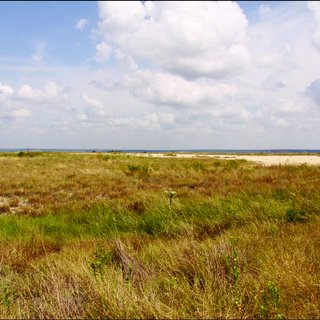
\includegraphics[height=1.0in, width=4in]{grassland.jpg}
	\end{center}
\end{frame}

\begin{frame}
	\frametitle{Cattle herds}

	30 head per herd, 464 herds, initialized at 116 corrals \\~\\

	Move around environment grazing according to ``win-switch'' strategy\\~\\

	Movement logic: pick cell with highest \textbf{grazing quality}
	\begin{itemize}
		\item \small Grazing suitability (per previous slide)
		\item \small Time since previous occupation
		\item \small Distance from current location \\~\\
	\end{itemize}

	Move after 8 days

	\begin{center}
		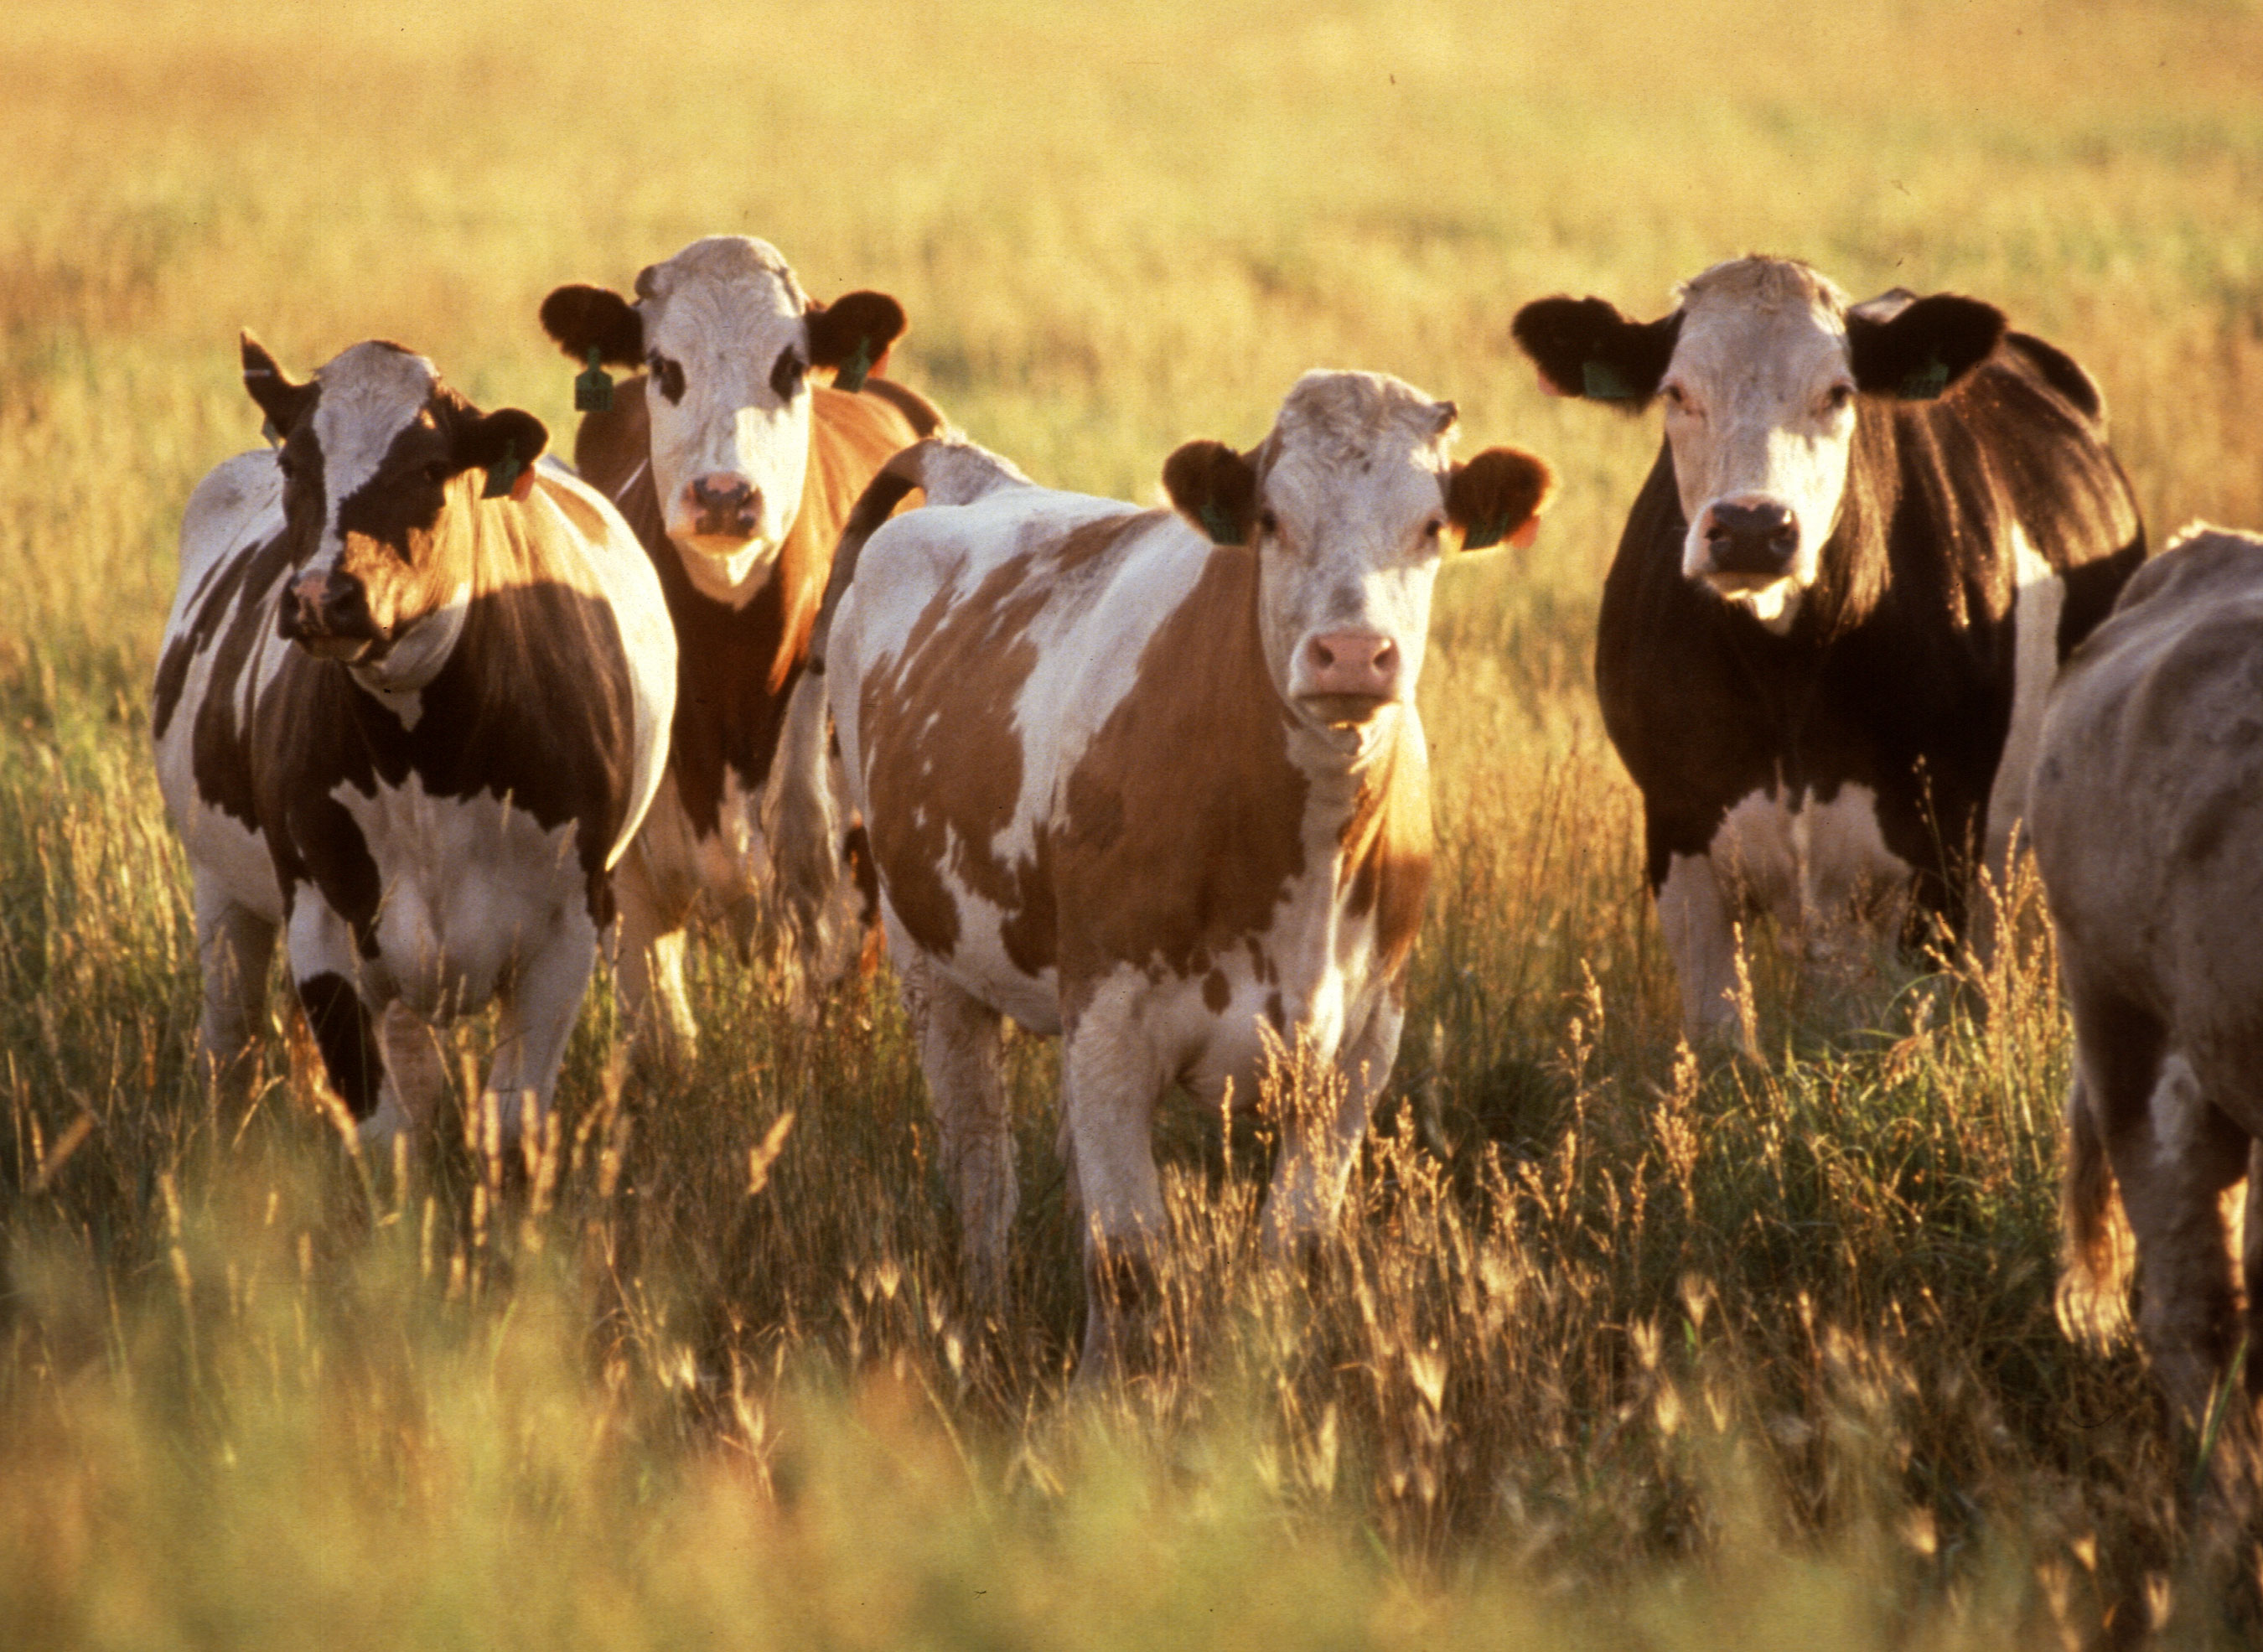
\includegraphics[height=1.0in, keepaspectratio]{herd.jpg}
	\end{center}
\end{frame}

\begin{frame}
	\frametitle{Cowbirds}

	Randomly initialized in breeding-area squares \\~\\

	Cognition for moving from breeding area to feeding area\\~\\

	Four possible movement rules 
	\begin{itemize}
		\item \small Next-nearest: move randomly to nearest feeding area until cows found
		\item \small Memory: try places have been before
		\item \small Memory-with-perception: add ability to assess feeding areas en-route
		\item \small Omniscient: benchmark\\~\\
	\end{itemize}
	\begin{center}
		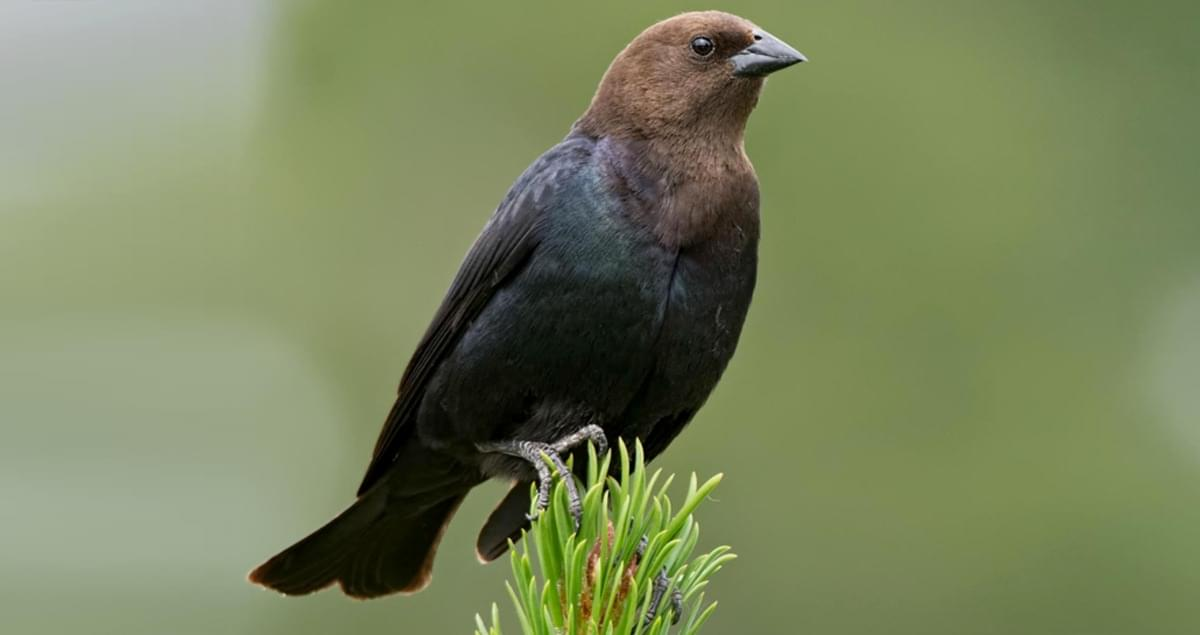
\includegraphics[height=1.0in, keepaspectratio]{bird.jpg}
	\end{center}
\end{frame}

\begin{frame}
	\frametitle{Trapping}
	Two new agent types \\~\\
	
	\textbf{Traps} 
	\begin{itemize}
		\item \small Can be mobile or fixed
		\item \small Occupy cell
		\item \small Have some probability of capturing a bird that visits cell \\~\\
	\end{itemize}
	
	\textbf{Trap managers}
	\begin{itemize}
		\item \small Goal: place traps where most cowbirds are
		\item \small Places traps and moves mobile ones
		\item \small Cognition for doing so is under-described
	\end{itemize}

	\begin{center}
		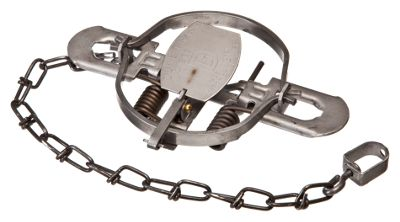
\includegraphics[height=1.0in, keepaspectratio]{trap.jpeg}
	\end{center}

\end{frame}

\begin{frame}
	\frametitle{V\&V and results}
	
	Parameter values well-justified and subjected to sensitivity analyses
	\begin{itemize}
		\item \small Field studies, literature review, etc.
		\item \small Many different runs with different settings (e.g. cowbird cognition) \\~\\
	\end{itemize}

	Simulation appears to qualitatively match real life \\~\\

	Fixed traps more effective (entirely based on parameter $p(\mathrm{catch)})$\\~\\

	Model-based trapping strategy caught 42\% more than real life strategy
\end{frame}

\begin{frame}
	\frametitle{Model effectiveness and course themes}

	In our taxonomy: analyzed-analyzed \\~\\

	In my opinion, one of the best models this semester
	\begin{itemize}
		\item \small Clear, scoped purpose (no \textit{exploration of potential} here!)
		\item \small Logical and well-justified modeling choices
		\item \small Solves real-world problem \\~\\
	\end{itemize}

	Somewhat depressing that best models (e.g. this and Yellowstone elk) are of animals with much more limited
	behavior space than humans \\~\\

	Course themes:
	\begin{itemize}
		\item \small ABM-GIS integration: serves as a great example of a problem that is nearly-intractable
			unless you include both elements and integrate
	\end{itemize}
\end{frame}

\end{document}
